\documentclass[9pt,times]{article}
%\usepackage{times}
%\usepackage{timesmath}
\newcommand{\w}{\omega}
\usepackage{epsfig}
%\newcommand{\psfig}[1]{}
\newcommand{\ignore}[1]{}

\begin{document}

\title{Generating stationary noise for noise simulation}
\author{J.~Roychowdhury}
\date{started sometime in 1996}

\maketitle

\begin{abstract}
Stationary noise sources are fundamental in noise analysis.
This work introduces a simple new method of generating
stationary noise for time-domain simulation, backed by a proof of
stationarity and analytic expressions for power spectral density.  The new
method is useful when stationarity and precisely-known
power-spectral-density functions are required for Monte-Carlo noise
simulation. Noise predictions using the theory are verified against
simulation results.
\end{abstract}

\section{Introduction}
\label{sec:intro}

%Why stationarity is important in noise sources.
%	Thermal noise is always stationary.
%	Shot noise is stationary if the diode current is steady.
% \subsection{Stationary noise sources}
{\em Stationary} stochastic processes play an important r\^ole in
noise analysis. Thermal noise generated by resistors, for example, is always
stationary; so is shot noise (in PN junctions) and flicker noise (in
MOSFETs) in devices with DC bias. Even when device biases are time-varying,
the noises generated in them are usually modelled as products of stationary
stochastic processes and deterministic time-varying waveforms\cite{reference}.

%Analysis of circuit noise
% 	fully stationary ac well-established, efficient algorithms.
% 	For cyclostationary, new theories and algorithms proposed.
% 		for their verification, Monte-Carlo useful.
%
%	Recently, theories and algorithms for cyclostationary noise have
%		been proposed that predict non-intuitive results. To
%		verify these theories and algorithms, Monte-Carlo
%		simulations need precisely-known stationary noise generators.
%	Also, if the noise is large enough to create nonlinear effects in
%		the circuit, Monte-Carlo is the only way.

Well-established analysis techniques exist for stationary noise
under quiescent biasses \cite{references}, based on frequency-domain linear
time-invariant small-signal analysis. When biases are time-varying, or if
noise levels are too large to be considered small perturbations, linear
time-invariant analyses do not suffice; Monte-Carlo simulation methods
\cite{rubinstein} are useful for analyzing noise in these situations.
Monte-Carlo simulation is also useful for verifying thories and algorithms
that have been proposed recently for calculating cyclostationary noise in
nonlinear systems \cite{newwork}. For such simulation to produce reliable
results, it is important to be able to generate stationary noise with a-priori 
known power spectral densities.

%What is the previous work; what are our advantages and disadvantages.
{
\subsection{Previous Work}
\ignore{
	Previous work
		0. Random vibration of mechanical and structural systems
		(T.T. Soong and Mircea Grigoriou), Prentice-Hall, 1993
			page 341:
			Approximate spectral representation: a. sum of closely
				spaced sinusoids with independent amplitudes
				coeffs of appropriate variances, b. sum of
				sinusoids of deterministic amplitudes and
				random phases. Good for ensemble averaging,
				but are they good for temporal averaging?
				clearly not. further are they stationary?
				need to check. maybe good for narrowband
				noise.
				a. is Gaussian if the amplitude r.v.s are
				Gaussian, but b. is not for a finite number
				of sinuosoids; however it tends to Gaussian
				as larger numbers of sinusoids are taken.
			Time-series models:
				ARMA models - autoregressive moving average
				- the output of i.i.d random variables
				applied to a difference equation. major
				problem: stationarity defined only w.r.t
				discrete samples. Does not provide
				stationarity in the sense of a continuous
				process.

		0.5: Broken line processes?

		1. Linear and nonlinear systems with non-gaussian white noise
		input (Mircea Grigoriu), Probabilistic Engg. Mechanics 10 (1995)
		171-179
			Talks about several methods for analyzing nonlinear
				systems with alpha-stable white noise (a
				generalization of gaussian white noise)
				Touches on Monte-Carlo in a discrete
				framework with a difference equation. These
				correspond to equispaced discretization of
				a differential equation.

		2. Reply to the "Comment on 'Numerical method for
		coloured-noise generation and its application to a bistable
		system'" (K.Y.R. Billah and M. Shinozuka), Phys. Rev. A, v46
		no. 12, 15 dec 1992
			Have not got hold of the original paper, which
			is in Phys. Rev. A 46, 8028 (1992)
		
		3. Parametric models of nonstationary Gaussian Processes (M.
		Grigoriou) Probabilistic Engg. Mechanics 10 (1995) 95-102
			3 ways of generating nonstationary gaussian
			processes: using polynomials, splines and a sampling
			theorem for stationary processes. all are
			finite sums of deterministic functions with random
			amplitudes which converge as the number of terms is
			increased. uses 2-dimensional psds.

		4. Simulation of nonstationary gaussian processes by random
		trigonometric polynomials (m. grigoriou), journal of engg.
		mechanics, vol 119, no 2, feb 1993, pp 328-343
			Uses a basis of trigonometric functions with random
			gaussian (and correlated) coefficients to generate
			nonstationary noise.

		5. Probabilistic models and simulation methods for seismic
		ground acceleration (m. grigoriou), Meccanicca 30: 105-124,
		1995.
			a review of probabilistic models of seismic ground
			acceleration (uniformly modulated, oscillatory,
			amplitude/phase modulated, ARMA); presents a novel
			nonstationary gaussian model. pages 114 and 115 talk
			a little about stationary noise generation; nothing
			new, all given in his book.

		6. Wavelet-Based Representations for the 1/f Family of
		Fractal Processes (Gregory W. Wornell), Proc. IEEE, vol 81
		no 10 october 1993 pp 1428-1450
			An excellent paper to read to get a good
			understanding of 1/f processes.
			talks about the 1/f family of fractal random
			processes, and the lack of convenient
			"representations" for these despite their apparent
			importance. Produces such a representation using
			wavelet bases. Says that 1/f processes have
			long-term correlation and cannot be generated by
			ARMA models. Several "useful", though not
			universally acceptable, characterizations already
			exist: 1. fractional integer formulation (Kolmogorov),
			2. extended/infinite-order ARMA models (van der Ziel),
			3. transmission line model (Keshner). Then he points
			out problems with these approaches. Then he points
			out what he is doing and its advantages; finally he
			outlines the format of the paper.
			He also has, on pages 1433 and 1435, explanations of
			what 1/f processes are, and how to characterize them
			mathematically. On page 1432, he has a list of physical
			situations in which 1/f processes arise.

		7. Simulation of stochastic processes by spectral
		representation (M. Shinozuka and G. Deodatis), Appl. Mech.
		Reviews 44(4), 1991, 191-203
			reference to this in 5. sent for.
	Why discrete i.i.d variables will not do - implicit
		interpolation in ODE solvers, adaptive timesteps disallowed,
		Stationarity not proven, PSD not precisely known a-priori.
	Our advantages
		single source + filter generates wide-band PSD.
		very little computation, and independent of width of PSD.
		preserves ergodicity in samples
		Non-uniform time-stepping is allowed.
		PSD precisely known, with expression.
		Stationarity can be obtained with even a very simple filter.
	Disadavantages:
		Can require large numbers of random variables if simulations
			are long.
		Coloured PSD can require complicated filters.
		If narrow band PSDs are required, there may be some more
			efficient way.
		Targetted towards time-domain Monte-Carlo; not towards
		frequency-domain Monte-Carlo, if that can be meaningfully
		defined.
}

Existing methods for generating samples of stationary noise use spectral
discretization, auto-regressive moving average (ARMA) models or broken-line
processes. Spectral discretization relies on approximating the process as a
finite sum of sinusoids with independent random amplitudes\cite{reference}.
A variation on this uses deterministic amplitudes but random
phases\cite{reference}. These methods define a continuous-time waveform and
require only a fixed number of random variables to generate each sample for
all time. ARMA methods generate discrete-time stationary noise by exciting a
linear difference equation with i.i.d random variables\cite{reference}. By
appropriate choice of the difference equation, different power spectral
densities can be synthesized.

%Our contributions
In this paper, a simple new way of generating stationary noise, useful for
time-domain Monte-Carlo simulation, is presented. It is proved that the new
technique produces stationary noise and analytic expressions for its power
spectral density are presented. Using only a single current source, resistor
and capacitor for each noise source, the technique is especially efficient
in generating wide-band noise. Simulation results are presented to verify
the new method and its power spectral density formulae.

Broken-line process - shifting creates ensemble averaging; filtering -
temporal and ensemble averaging. Generalization of ARMA to continuous time.
Simple interpretation in the frequency domain of the condition required for
averaging to produce stationary noise.

Issues: 1. Stationarity, 2. Whiteness, 3. Ergodicity, 4. ramp-up time
	to asymptotic stationary value, 5. gaussianness.

Paper organization: The model and theoretical analysis using cyclostationary
noise concepts, choice of parameters and numerical calculations,
verification against Monte-Carlo, step-by-step procedure for
designing your own stationary noise source, conclusion.
}

\section{Generating Stationary White Noise in the Time Domain -- Theory}
\label{sec:theory}
The noise source is generated by linear interpolation of a uniformly spaced
sequence of independent Gaussian sources each of variance 1. The spacing
between the sources is T.

\ignore{
It is immediate that the autocorrelation function
of this sequence is a symmetric hat on [-T, T] (going from 0 at -T linearly
to 1 at 0 and down again to 0 at T). The PSD is the Fourier
transform of this function $f(t)$. Note that $f(t)$ is even, and equal to
$1-{t\over T}$ for $0\le t\le T$.

This is:
\begin{eqnarray*}
\int_{-T}^T f(t) e^{j\w t} \, dt & = & 2 \int_0^T f(t) \cos(\w t) \, dt \\
	& = & {2\over\w}\sin(\w T) - {2\over T}\int_0^T t\cos(\w t)\,dt \\
	& = & {2\over\w}\sin(\w T) - {2\over T} {\left[ {t\over\w}\sin(\w t)
	      - {1\over\w}\int\sin(\w t)\,dt \right]}_0^T \\
	& = & {2\over\w}\sin(\w T) - {2\over T} {\left[ {t\over\w}\sin(\w t)
	      + {1\over\w^2}\cos(\w t) \right]}_0^T \\
	& = & {2\over\w}\sin(\w T) - {2\over T} \left[{T\over\w}\sin(\w T)
	      + {1\over\w^2}\cos(\w T)\right] + {2\over \w^2 T}\\
	& = & {2\over\w^2 T}\left[ 1-\cos(\w T)\right]\\
\end{eqnarray*}

Applying L'Hospital's rule, the limit of this as $\w \to 0$ is $T$, as
expected. When plotted, it looks like a sinc as a function  of $\w$. The
value stays substantially flat upto $\w \approx {1\over 10T}$.
Figures~\ref{fig:linear} and~\ref{fig:loglinear} demonstrate this.
\begin{figure}[htbp]
\centerline{\ 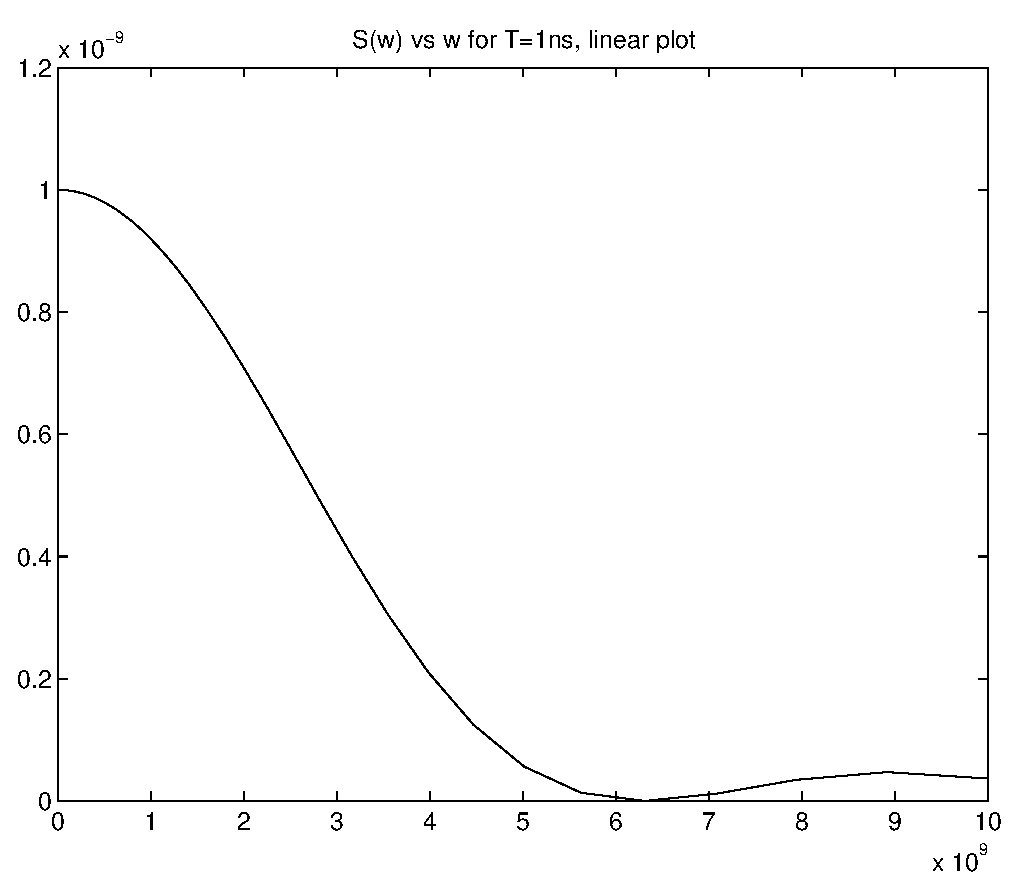
\psfig{file=./figs/inpnoise1.ps,width=0.7\textwidth}}
\caption{}
\label{fig:linear}
\end{figure}
\begin{figure}[htbp]
\centerline{\ 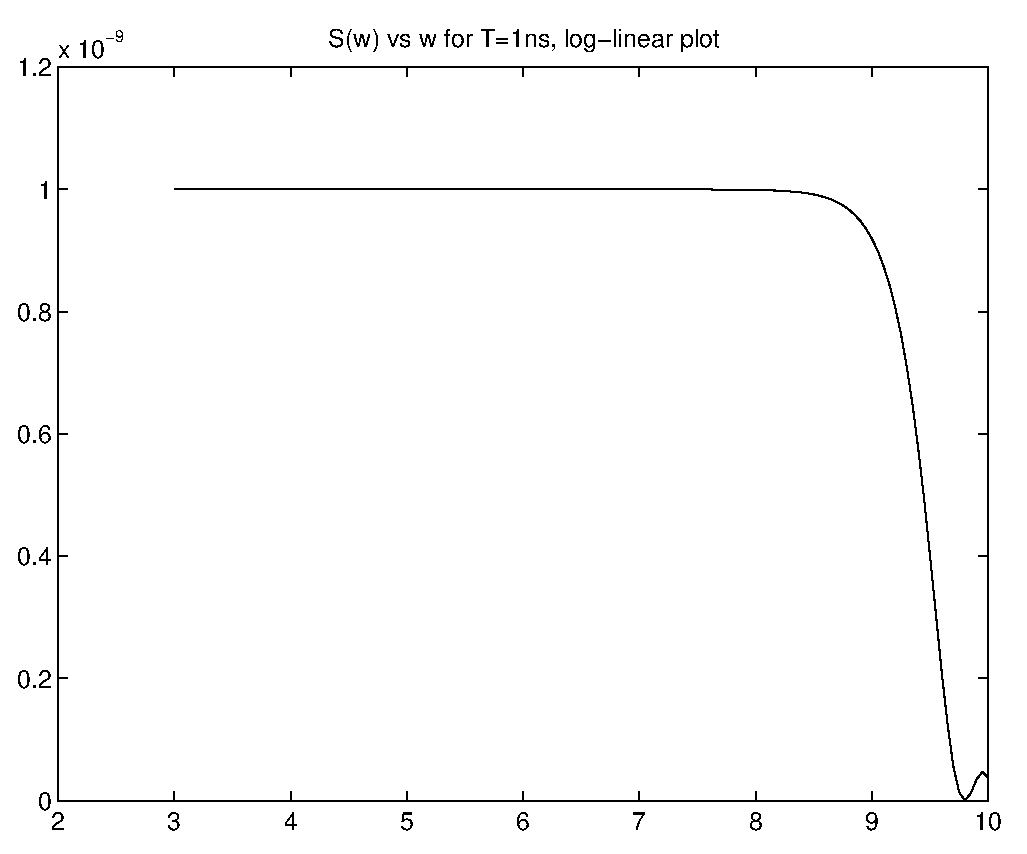
\psfig{file=./figs/inpnoise2.ps,width=0.7\textwidth}}
\caption{}
\label{fig:loglinear}
\end{figure}

All this is fine but probably of limited use, because the process unfortunately
is not stationary.
}

Consider the autocorrelation function
$R(t,\tau) = E[x(t)x(t+\tau)]$. 
Now $x_1 = x(t) = \left(1-{t\over T}\right)n_1 + {t\over T}n_2$, 
where $n_1$ and $n_2$
are the independent noise sources at time $0$ and $T$. If $t <= T - \tau$,
then $x_2 = \left(1-{t+\tau\over T}\right)n_1 + {t+\tau\over T}n_2$; if $
T-\tau \le t \le T$, $x_2 = \left(1-{t+\tau-T\over T}\right)n_2 +
{t+\tau-T\over T}n_3$. Here $t \in [0,T]$. Then
\[
R(t,\tau) = \cases{ 
	\left(1-{t\over T}\right)\left(1-{t+\tau\over T}\right)
		+ {t\over T}{t+\tau\over T}
			& if $-t\le\tau\le T-t$;\cr
	{t\over T}\left(1-{t+\tau-T\over T}\right)
			& if $T-t\le\tau\le 2T-t$;\cr
	0
			& if $2T-t\le\tau$;\cr
	\left(1-{t\over T}\right)\left(1+{t+\tau\over T}\right)
			& if $-T-t\le\tau\le-t$;\cr
	0
			& if $\tau\le-T-t$.
}
\]
If $\tau$ is fixed, the autocorrelation is
$T$-periodic in $t$. For $0\le t\le T$, fix $\tau$ at a given value, and
rewrite the above to show better the variation with $t$:
\[
R(t,\tau) = \cases{ 
	0
			& if $t\le-T-\tau$;\cr
	\left(1-{t\over T}\right)\left(1+{t+\tau\over T}\right)
			& if $-T-\tau\le t\le-\tau$;\cr
	\left(1-{t\over T}\right)\left(1-{t+\tau\over T}\right)
		+ {t\over T}{t+\tau\over T}
			& if $-\tau\le t\le T-\tau$;\cr
	{t\over T}\left(1-{t+\tau-T\over T}\right)
			& if $T-\tau\le t\le 2T-\tau$;\cr
	0
			& if $2T-\tau\le t$.
}
\]
$R(t,\tau)$ is plotted in Figure~\ref{fig:Rttau} ($T=1$).
\begin{figure}[htbp]
\centerline{\ \psfig{file=./figs/Rttau.ps.gz,width=0.7\textwidth}}
\caption{}
\label{fig:Rttau}
\end{figure}

We want to expand $R(t,\tau)$ in a Fourier series in $t$. We are interested
in particular in the DC component of the Fourier series since it is the
stationary component. Hence for a fixed $\tau$, we need to find the average
value of $R(t,\tau)$ over $t \in [0,T]$. To do this, we look at
$R(t,\tau)$ over segments of $\tau$:

\[
R(t,\tau) = \cases{
	0
		& if $\tau<-2T$;\cr
	\cases{
		0 
			& if $0\le t\le-T-\tau$;\cr
		\left(1-{t\over T}\right)\left(1+{t+\tau\over T}\right)
			& if $-T-\tau\le t\le T$.
	} 
		& if $-2T\le\tau\le-T$; \cr
	\cases{
		\left(1-{t\over T}\right)\left(1+{t+\tau\over T}\right)
			& if $0\le t\le -\tau$;\cr
		\left(1-{t\over T}\right)\left(1-{t+\tau\over
					T}\right)+{t\over T}{t+\tau\over T}
			& if $-\tau\le t\le T$.
	} 
		& if $-T\le\tau\le 0$; \cr
	\cases{
		\left(1-{t\over T}\right)\left(1-{t+\tau\over
					T}\right)+{t\over T}{t+\tau\over T}
			& if $0\le t\le T-\tau$;\cr
		{t\over T}\left(1-{t+\tau-T\over T}\right)
			& if $T-\tau\le t\le T$.
	} 
		& if $0\le\tau\le T$; \cr
	\cases{
		{t\over T}\left(1-{t+\tau-T\over T}\right)
			& if $0\le t\le 2T-\tau$;\cr
		0
			& if $2T-\tau\le t\le T$.
	} 
		& if $T\le\tau\le 2T$; \cr
	0
		& if $\tau \ge 2T$.
}
\]

Taking the average over $t \in [0,T]$, we get
\[
R_0(\tau) = \cases{
	0
		& if $\tau<-2T$;\cr
	{1\over T}\left( {\frac {12\,\tau\,T^{2}+8\,T^{3}+6\,
				T\tau^{2}+\tau^{3}}{6\,T^{2}}}\right)
		& if $-2T\le\tau\le-T$; \cr
	{1\over T}\left( -{\frac {\tau\,\left (6\,T^{2}+\tau^{2}+6\,
				T\tau\right )}{6\,T^{2}}} + 
				{\frac {2\,T^{3}-\tau^{3}+3\,\tau\,T^{2}}
				{3\,T^{2}}} \right)
		& if $-T\le\tau\le 0$; \cr
	{1\over T}\left( {\frac {2\,T^{3}-3\,\tau\,T^{2}+\tau^{3}}{3\,T^{2}}}+
				{\frac {\tau\,\left (6\,T^{2}-6\,T\tau+
				\tau^{2}\right)}{6\,T^{2}}} \right)
		& if $0\le\tau\le T$; \cr
	{1\over T}{\frac {\left (2\,T-\tau\right)^{3}}{6\,T^{2}}}
		& if $T\le\tau\le 2T$; \cr
	0
		& if $\tau \ge 2T$.
}
\]
This function is plotted in Figure~\ref{fig:R0tau} ($T=1$):
\begin{figure}[htbp]
\centerline{\ 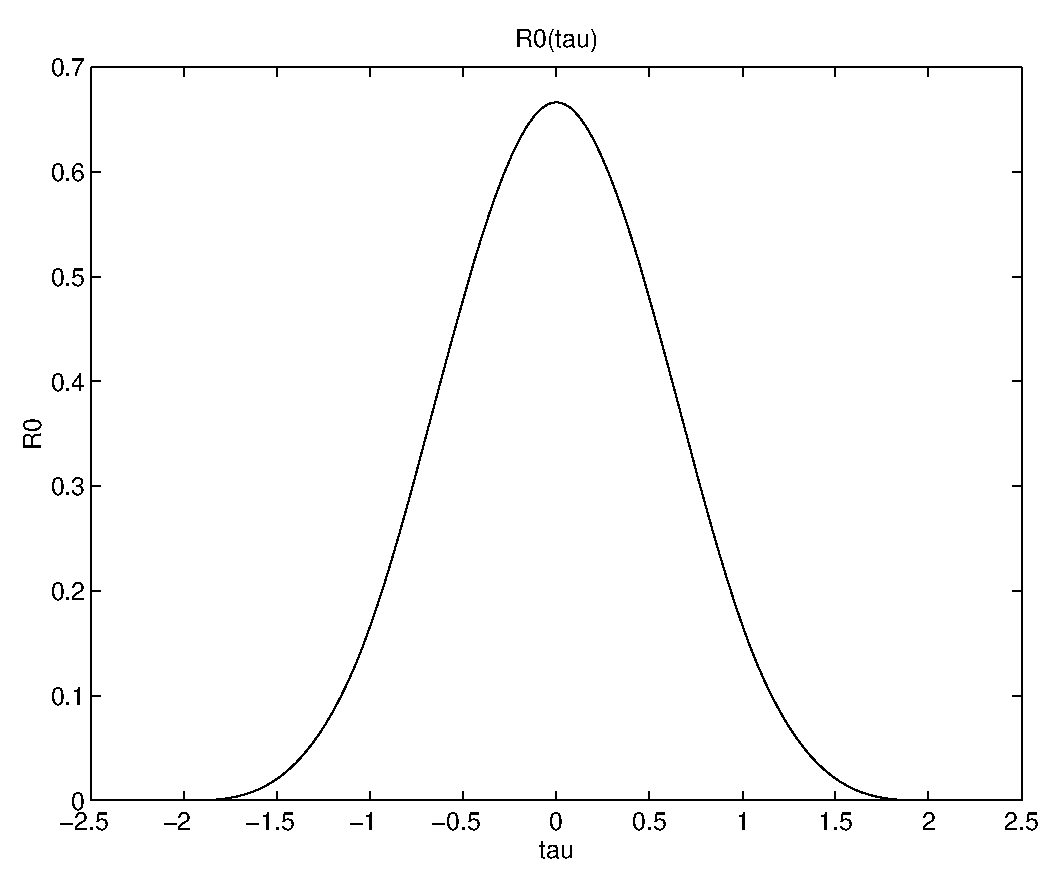
\psfig{file=./figs/R0tau.ps,width=0.7\textwidth}}
\caption{}
\label{fig:R0tau}
\end{figure}
The stationary power spectral density $S_0(\w)$ is the Fourier transform of
$R_0(\tau)$, given by:
\[
S_0(\w) =
-{\frac {8\,\cos(T\omega)-2\,\cos(2\,T\omega)-6}{\omega^{4}T^{3}}}
\]
As $\w\to0$, $S_0(\w)\to T$. $S_0(\w)$ for $T=1$ns is shown in
Figures~\ref{fig:S0loglin} and~\ref{fig:S0linear}.
\begin{figure}[htbp]
\centerline{\ 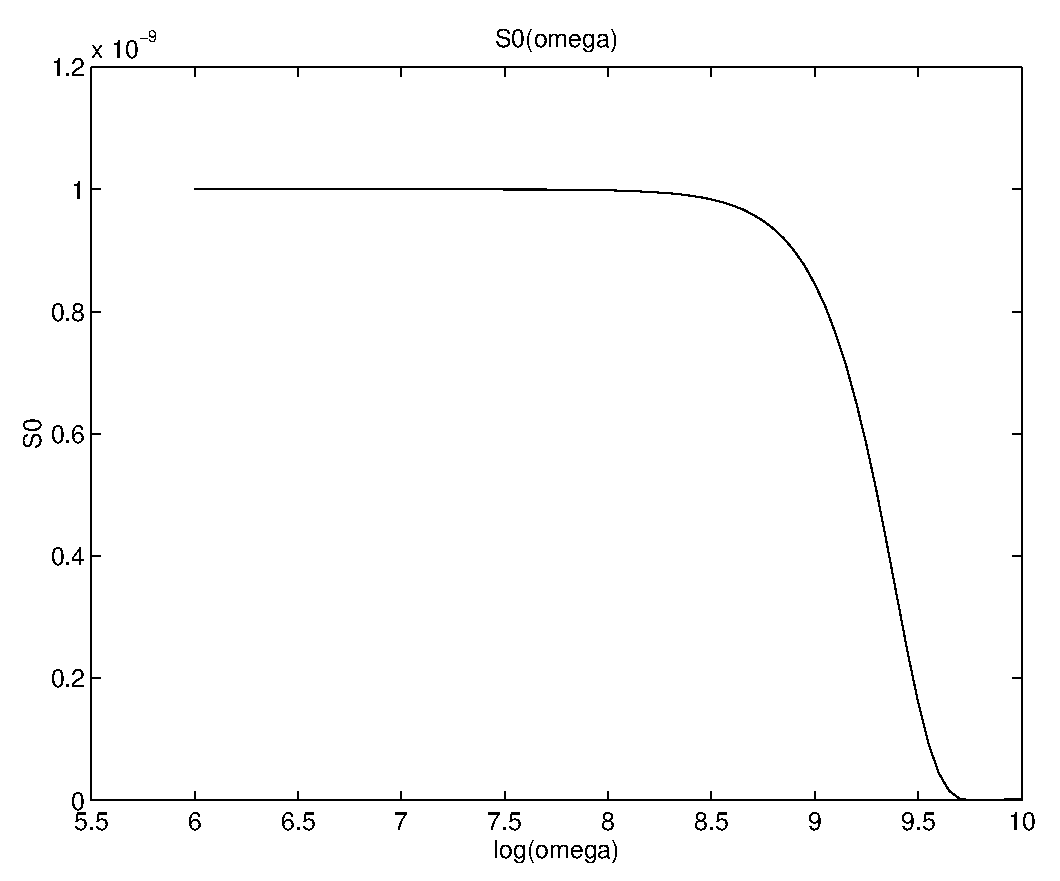
\psfig{file=./figs/S0loglin.ps,width=0.7\textwidth}}
\caption{}
\label{fig:S0loglin}
\end{figure}
\begin{figure}[htbp]
\centerline{\ 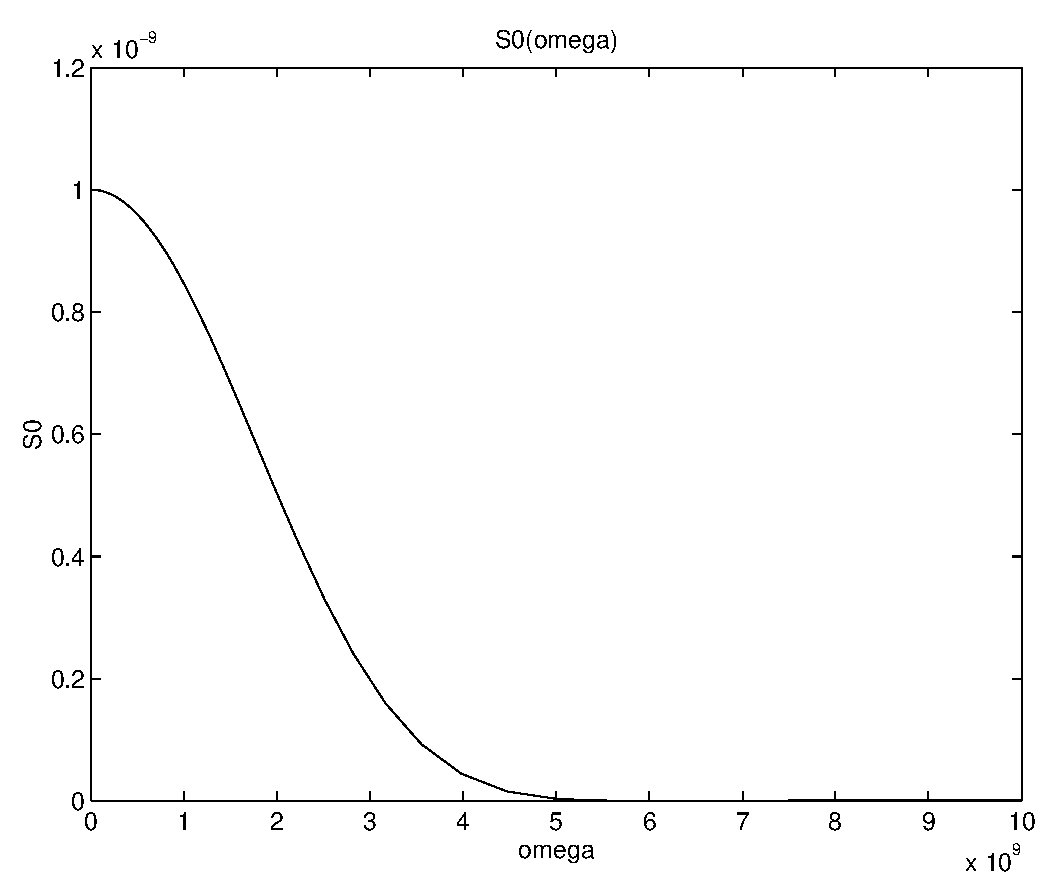
\psfig{file=./figs/S0linear.ps,width=0.7\textwidth}}
\caption{}
\label{fig:S0linear}
\end{figure}

Stationarity can be achieved simply by translating the grid of sample points
randomly (uniform distribution over $[0,T]$).
Alternatively, if this cyclostationary source is sent
through a low-pass filter of bandwidth less that $1\over 2T$, then all
higher-order PSDs $S_i, i\ne 0$ will be completely killed and only $S_0$
will be passed. Hence the output noise will be stationary, and {\em if the
filter bandwidth is less than $1\over 100T$ or so, the cyclostationary
source will look like a stationary white noise source with a flat PSD of
$T$}.

\section{Numerical Calculations}
\label{sec:numcalc}
For a current source of unit variance feeding a resistor in parallel with a
capacitor, we have $H(s) = {R\over 1+sRC}$, $H(f) = {R\over 1+j2\pi fRC}$.
$\int \left| H(f) \right|^2 \,df= {R\over 2\pi C}\tan^{-1}(2\pi R C f)$,
hence $\int_{-\infty}^{\infty} \left| H(f) \right|^2 \,df = {R\over 2 C}$.
Thus the variance of the voltage generated is approximately $R T \over 2 C$
- this is an upper bound.

More accurately, we have
\begin{eqnarray}
\label{eq:whitesourcevariance}
R_0(0) & = & \int_{-\infty}^\infty \left|H(f)\right|^2 S_0(f) \, df \nonumber \\
       & = & - \int_{-\infty}^\infty \left|{R\over 1+j2\pi fRC}\right|^2 {\frac
       {8\,\cos(2\pi f T)-2\,\cos(4\pi f T)-6}{{(2\pi f)}^{4}T^{3}}} \, df
       \nonumber\\
       & = & - \int_{-\infty}^\infty {R^2\over 1+4\pi^2 f^2R^2C^2}{\frac
       {8\,\cos(2\pi f T)-2\,\cos(4\pi f T)-6}{{(2\pi f)}^{4}T^{3}}} \, df 
\end{eqnarray}

This integral is difficult to evaluate analytically (i.e., {\sf maple} has
trouble) so we have to resort to numerical integration for given values of
$R$, $C$ and $T$. For the mixer and filter combination circuit in 
{\sf doc/noise/montecarlo/mixerfilter}, the following values are used:
\[
R=1\Omega, \qquad C=5\mu F,\qquad T=1\mu s
\]
The RC pole is at $200\over 2\pi$KHz. The square of the transfer function
magnitude is shown in Fig.~\ref{fig:magH2}.
\begin{figure}[htbp]
\centerline{\ 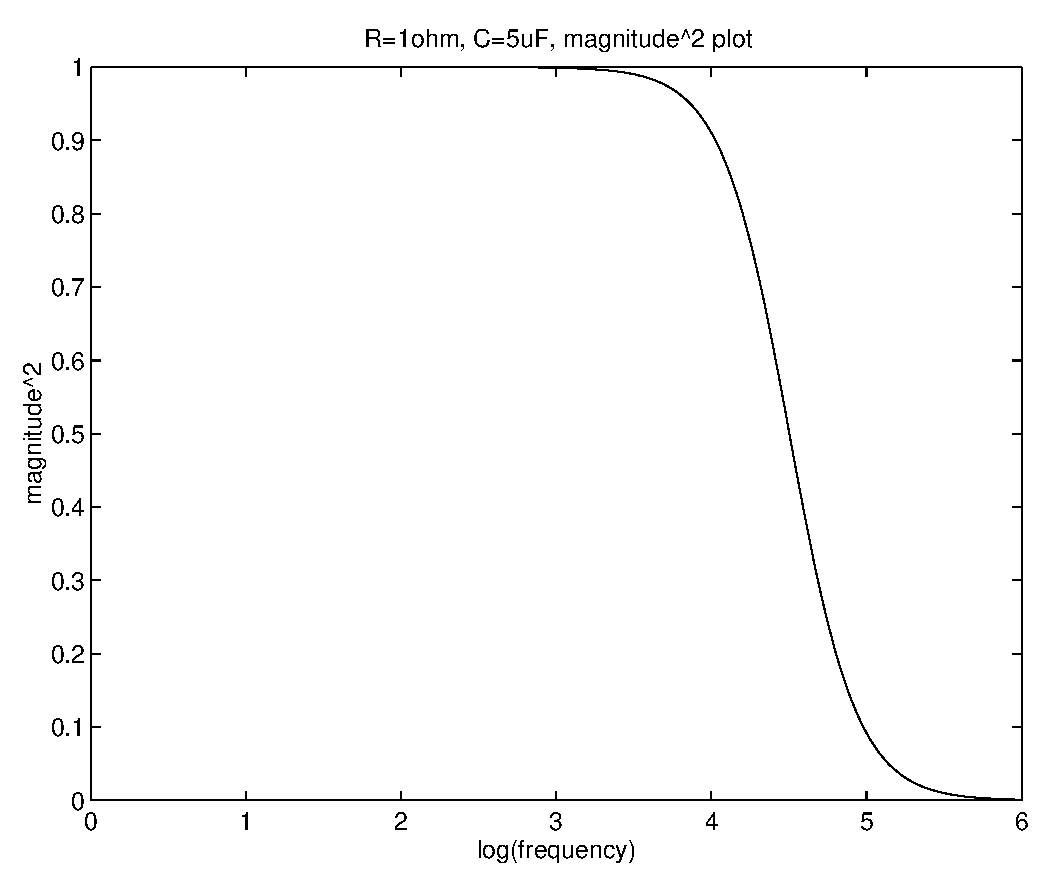
\psfig{file=./figs/magH2.ps,width=0.7\textwidth}}
\caption{}
\label{fig:magH2}
\end{figure}
The integrand of Equation~\ref{eq:whitesourcevariance} is shown in
Figure~\ref{fig:}. When integrated numerically  over the interval $[-10^7,
10^7]$ (using {\sf maple}), we get a result of 0.0912 for $R_0(0)$, the
stationary variance. The upper-bound $R T \over 2 C$ equals 0.1;
hence we see that in this case, the rolloff of $S_0(\w)$ makes a difference of
about 10\% to the variance.

\section{Verification against Monte-Carlo Simulations}
\label{sec:montecarlo}

Brute-force Monte-Carlo simulations were performed in order the verify the
above predictions. The Monte-Carlo simulations were designed to estimate, as
a function of time, the variance of the output noise generated by passing a
linearly interpolated comb of i.i.d gaussian random variables of unit
variance, with comb spacing T, through an RC filter. Two basic approaches
were taken to simulating this system: 1. solving the differential equation
numerically using a general-purpose numerical integration method, and 2.
using the fact that the differential equation for a RC network driven by a
PWL current source can be integrated analytically, and applying the formulae
thus obtained. The values of R, C and T were the same as in
Section~\ref{sec:numcalc}.

The first approach, solving the differential equation numerically, was tried
using the internal circuit simulator ADVICE. A sample size of 10,000 input
waveforms was chosen initially, each extending to a length of 5 RC
time-constants (200us). This translated to an execution time of
about 1 month on a Sun SparcStation 20; this being impractical, the sample
size was reduced to 1000 and the simulations were completed in three days.
The outputs were postprocessed to obtain the noise variances. The variances
of the PWL current source and the filtered output voltage, plotted over a
period $30T$ at the end of the simulation, are shown in
Figures~\ref{fig:iin-rc-advice} and~\ref{fig:v1-rc-advice}. The
cyclostationary change of the variance of the input current source, between
1.0 and 0.5, can be seen in Figure~\ref{fig:iin-rc-advice}; it
is also evident, from Figure~\ref{fig:v1-rc-advice}, that no such
cyclostationary variation exists for filtered output voltage variance, which
wanders between approximately 0.086 and 0.1 on a scale much coarser than
T=1us.  (The circuit and results for this experiment are in
{\sf doc/noise/montecarlo/mixerfilter-advice}.)

\begin{figure}[htbp]
\centerline{\ \psfig{file=./figs/iin-rc-advice.ps,width=0.7\textwidth}}
\caption{1000 ADVICE simulations: variance of input current source wrt time}
\label{fig:iin-rc-advice}
\end{figure}
\begin{figure}[htbp]
\centerline{\ \psfig{file=./figs/v1-rc-advice.ps,width=0.7\textwidth}}
\caption{1000 ADVICE simulations: variance of RC-filtered output voltage wrt time}
\label{fig:v1-rc-advice}
\end{figure}

Since the 1000 samples in the experiment above were not enough to verify
conclusively the theoretically predicted output noise variance of 0.0912
(from Section~\ref{sec:numcalc}), 10000 samples were tried next. To avoid
the excessive computation time needed by ADVICE, a custom program was
written in C/C++ to perform numerical integration of the circuit's
differential equation. A fourth-order Runge-Kutta method (using the
Numerical Recipes routine {\sf odeint}) was used. The simulation took about
10 hours of computer time. The variances of the input current and output
filtered voltage, as functions of time, are shown in
Figures~\ref{fig:iin-odeint-rc},~\ref{fig:v1-odeint-rc-wide}
and~\ref{fig:v1-odeint-rc-narrow}. It can be seen that the output variance
is stationary, at a value between about 0.088 and 0.095, or centered around
0.0915, close to the predicted value of 0.0912.

\begin{figure}[htbp]
\centerline{\ \psfig{file=./figs/iin-odeint-rc.ps,width=0.7\textwidth}}
\caption{10000 {\sf odeint} simulations: variance of input current source wrt time}
\label{fig:iin-odeint-rc}
\end{figure}
\begin{figure}[htbp]
\centerline{\ \psfig{file=./figs/v1-odeint-rc-wide.ps,width=0.7\textwidth}}
\caption{10000 {\sf odeint} simulations: variance of RC-filtered output voltage wrt time}
\label{fig:v1-odeint-rc-wide}
\end{figure}
\begin{figure}[htbp]
\centerline{\ \psfig{file=./figs/v1-odeint-rc-narrow.ps,width=0.7\textwidth}}
\caption{10000 {\sf odeint} simulations: variance of RC-filtered output
		voltage wrt time (detail)}
\label{fig:v1-odeint-rc-narrow}
\end{figure}

To obtain a more precise estimate, the number of sample waveforms was
increased to 100000. In order to reduce the simulation time and increase
accuracy of results, the second approach mentioned above was tried.  A
program based on analytic expressions for the ODE solution when excited with
a PWL source, was used (the code is in {\sf doc/noise/montecarlo/rc-in-c++}).
This program took about 30 minutes to execute. The input and output
variances are shown in Figures~\ref{fig:iin-analytic-rc}
and~\ref{fig:v1-analytic-rc}. The output variance is again stationary,
between about 0.090 and 0.0925, or centered around 0.0915, again close to
the predicted value of 0.0912.

\begin{figure}[htbp]
\centerline{\ \psfig{file=./figs/iin-analytic-rc.ps,width=0.7\textwidth}}
\caption{100000 analytic simulations: variance of input current source wrt time}
\label{fig:iin-analytic-rc}
\end{figure}
\begin{figure}[htbp]
\centerline{\ \psfig{file=./figs/v1-analytic-rc.ps,width=0.7\textwidth}}
\caption{100000 analytic simulations: variance of RC-filtered output voltage wrt time}
\label{fig:v1-analytic-rc}
\end{figure}

The above Monte-Carlo experiments verify the stationarity of the output
noise and provide a figure for the stationary noise variance that is
consistent with the theory of the previous sections. Another important
property of stationary processes is {\em ergodicity},
i.e., the condition that time-averages of each sample of the stationary
process equal ensemble averages at any time. 
To verify ergodicity, simulations using the analytic formulae were carried out 
for a length of about 40000 RC time-constants and the average power at the
output of the filter
computed\footnote{Note that a simulation of many times the RC time constant,
i.e., the time-period of correlation in the process, is necessary to obtain
results meaningful for ergodicity.}. Values for this average power from 5
runs (5 samples from the ensemble) were 0.09128, 0.09124, 0.09114, 0.09110
and 0.09104, matching closely the value predicted by theory in
Section~\ref{sec:numcalc} and the ensemble-average variance obtained from
Monte-Carlo simulation.
% more: 0.0916, 0.0910, 0.0914, 0.0913, 0.0914, 0.09096

\section{Conclusion}

\end{document}
